\section{Syntax | Dependency Parsing}
\subsection*{Description}
\emph{Task} --- 
Assign syntactic structure to a string by breaking it down into a hierarchy of dependencies (similar to syntactic parsing)

{\color{black}\hrule height 0.001mm}

\subsection*{Formulation}
\begin{itemize}
    \item String $w$
    \item \emph{Spanning tree}: 
    \begin{itemize}
        \item Connects $N$ nodes via $N-1$ edges
        \item Contains no cycles
        \item Number of nodes can be given by number of words in sentence $|w| = N$ or, if there are dependency parsing rules available, by number of items in the dependency rules (counting each item before and after the $\to$ separately, excl. the root, e.g. $\textrm{ROOT}\to\textrm{foo}, \textrm{foo}\to\textrm{bar},\textrm{foo}\to\textrm{baz}$ has 5 nodes)
    \end{itemize}
    \item For dependency parsing, we also require:
    \begin{itemize}
        \item The tree has exactly one root node, with only one outgoing edge
        \item All non-root nodes have exactly one incoming edge
        \item Edges are directed
        \item Edges are labeled
    \end{itemize}
    \item We can turn syntactic parsing into dependency parsing based on rules:
    \begin{itemize}
        \item Head of a production rule in syntactic parsing is the head of the dependency relation in dependency parsing
        \item Then, an arrow goes from the head to the sibling
        \item Then, weight for the given production rule in syntactic parsing is the weight assigned to the head-sibling dependency in dependency parsing
        \item E.g. in $NP \to Adj N$, $N$ is the head, so there is an arrow from $N$ to $Adj$
    \end{itemize}
    \item Types of dependency trees:
    \begin{itemize}
        \item \emph{Projective trees}:
        \begin{itemize}
            \item No crossing arcs
            \item Closely related to constituents (syntactic parsing)
            \item Note: In syntactic parsing, dependency relationships are always nested within constituents, meaning that syntactic parsing trees are always projective
        \end{itemize}
        \item \emph{Non-projective trees}:
        \begin{itemize}
            \item Crossing arcs
            \item In focus in the following
        \end{itemize}
    \end{itemize}
\end{itemize}

{\color{lightgray}\hrule height 0.001mm}

\emph{Probability of spanning tree} ---
\begin{itemize}
    \item 
    $
    p(t \mid w) = \frac{\exp(\textrm{score}(t, w))}{Z} = \frac{\exp(\textrm{score}(t, w))}{\sum_{t'} \exp(\textrm{score}(t', w))}
    $
    \item Challenge: Naively:
    \begin{itemize}
        \item There are $N^N$ undirected trees in graph if we don't impose a spanning tree structure and every node can depend on any other node, including itself, meaning it takes $\mathcal{O}(N^N)$ time to compute $Z$ 
        \item \emph{Cayley's formula}: There are $N^{N-2}$ undirected trees in graph if we impose a spanning tree structure constraint, meaning it takes $\mathcal{O}(N^{N-2})$ time to compute $Z$
        \item There are $(N-1)^{N-2}$ undirected trees in graph if we also impose the constraint that there is exactly one root node, meaning it takes  $\mathcal{O}((N-1)^{N-2})$ time to compute $Z$
    \end{itemize}
    \item Solution: 
    \begin{itemize}
        \item \emph{Edge factored assumption}:
        \begin{itemize}
            \item $
            p(t \mid w) = \frac{\prod_{(i \to j) \in t} \exp(\textrm{score}(i, j, w)) \exp(\textrm{score}(r, w))}{Z} = \frac{\prod_{(i \to j) \in t} \exp(\textrm{score}(i, j, w)) \exp(\textrm{score}(r, w))}{\sum_{t'} \prod_{(i \to j) \in t'} \exp(\textrm{score}(i, j, w)) \exp(\textrm{score}(r, w))}
            $ where $(i \to j)$ is an edge in the tree, $r$ is the root 
            \item Sp, in the denominator, we sum over the number of trees ($N^{N-2}$), and in the score, we sum over the number of edges ($N-1$)
            \item In edge factored assumption, scoring function $\textrm{score}(t, w)$ can only consider features that only depend on the edge $(i \to j)$ (e.g. length $|i-j|$) or do not depend on the edges at all (e.g. length of $\boldsymbol{w}$, tags of $w_i, w_j$, embeddings of $w_i, w_j, \boldsymbol{w}$, identity of words $w_i, w_j$), but not features that depend on other edges (e.g. higher-order dependency parsing, assigned root)
        \end{itemize}
        \item \emph{Kirchhoff's Matrix-Tree Theorem}: Method for counting the number of undirected spanning trees in $\mathcal{O}(N^3)$ time
        \item \emph{Tutte's Matrix-Tree Theorem}: Generalizes Kirchhoff's Matrix-Tree Theorem to directed spanning trees:
        \begin{itemize}
            \item Take adjacency matrix and root vector:
            \begin{itemize}
                \item \emph{Adjacency matrix}: One entry for each node $i$ to node $j$, if they were connected via an edge $i \to j$
                $
                A_{ij} = \exp(\textrm{score}(i, j, w))
                $
                with 0 on diagonal and not-null on off-diagonal
                \item \emph{Root vector}: One entry for each node $j$, if it were the root node
                $
                \rho_j = \exp(\textrm{score}(j, w))
                $
            \end{itemize}
            \item Construct \emph{Laplacian matrix}:
            Not accounting for constraint that there is only one root node:
            $L_{ij} =
            \begin{cases}
                -A_{ij} & \text{if } i \neq j \\
                \rho_j + \sum_{k \neq i} A_{kj} & \text{otherwise}
            \end{cases}$\\
            Accounting for constraint that there is only one root node:
            $L_{ij} =
            \begin{cases}
                \rho_j & \text{if } i = 1 \\
                \sum_{i'=1,i' \neq j}^n A_{i'j} & \text{if } i = j \\
                -A_{ij} & \text{otherwise}
            \end{cases}$
            i.e. 
            $\begin{cases}
                \text{- first row of L contains root scores} \\
                \text{- diagonal of L (except } L_{1,1} \text{) contains}\\
                \text{sum within each column of } A \text{ (except } A_{i,i} \text{)}\\
                \text{- off-diagonal of L (except first row) contains}\\ \text{elements of A multiplied with $-1$ }
            \end{cases}$
            \item According to matrix tree theorem: $|L| = \det(L) = Z =$ number of trees in graph
            \item According to Cayley's formula: number of undirected spanning trees in graph = $N^{N-2}$
        \end{itemize}
        \item Then, we can compute $Z$ under the edge factored assumption in $\mathcal{O}(N^3)$
    \end{itemize}
\end{itemize}

{\color{black}\hrule height 0.001mm}

\subsection*{Optimization}
Construct tree:
\begin{itemize}
    \item $N$ nodes plus 1 extra root node
    \item $N-1$ edges, of which $1$ edge is fixed (root) 
    \item Number of directed spanning trees: $N^{(N-1)}$
    \item Number of directed spanning trees, including labeling of edges: $N^{(N-1)} \times x$ where $x$ is given by the number of the destination nodes (e.g. $N$) raised to the power of the number of edges that can vary (e.g. $N-1-1 = N-2$), i.e. $N^{(N-2)}$
\end{itemize}

Decode tree:
\begin{itemize}
    \item Challenge: To perform decoding, greedy \emph{Kruskal's algorithm} does not work, since this selects the highest-scoring edge at each steps, which may be suboptimal in the directed case
    \item Solution: \emph{Chu-Liu/Edmonds algorithm}
\end{itemize}

\emph{Chu-Liu/Edmonds algorithm}:
\begin{itemize}
    \item Algorithm:
    \begin{enumerate}
        \item Greedy algorithm selects best incoming edge for each node, except the root
        \item This can cause cycles, which we need to contract:
        \begin{itemize}
            \item Cycle treated as one node
            \item Edges between nodes in the cycle are \textcolor{gray}{dead}
            \item Edges between nodes fully outside the cycle are \textcolor{teal}{external}
            \item Edges exiting the cycle are \textcolor{blue}{exits}
            \item Edges entering the cycle are \textcolor{magenta}{enters}
        \end{itemize}
        \item Break cycle: For each enter edge, break cycle by removing edges that are also incoming at the node where the enter edge is incoming
        \item Re-weight: To enter edge, add weights of remaining edges that are strictly on (not in) the cycle
        \item Now, greedy algorithm selects tree without cycles
        \item Then, we can re-expand: Pick edge of highest-scoring enter edge in contracted form, pick edges that were used to re-weight when breaking cycle on that enter edge
    \end{enumerate}
    \item Without root constraint: Can be run in $\mathcal{O}(N^2)$ time
    \item With root constraint:
    \begin{itemize}
        \item Naively: Run above algorithm $N$ times, fixing each edge as the only one emanating from the root, adds factor $N$ to runtime
        \item Solution: Adjusted algorithm
    \end{itemize}
    \item Adjusted algorithm:
    \begin{enumerate}
        \item Run steps $1-4$ (contract cycle, break cycle, re-weight edges) as above
        \item If there are multiple edges emanating from the root: For each root edge, calculate cost of deleting this edge: Cost = Weight of root edge - weight of next-best incoming edge to target node (treating any cycles as single nodes)
        \item Preliminarily remove edge with lowest cost, but keep target node intact
        \item Preliminarily repeat step $2$ (calculate root edge cost, remove lowest-cost root edge) here as needed
        \item Re-run greedy algorithm in contracted form
        \item If this leads to a cycle: Undo removal of edge with lowest cost, contract (treating any cycles as single nodes), then re-expand\\
        Otherwise: Re-expand
    \end{enumerate}
\end{itemize}

{\color{black}\hrule height 0.001mm}

\subsection*{Other}
\emph{First vs. second-order dependency parsing} ---
\begin{itemize}
    \item Above, we have considered first-order dependency parses only, but this can be extended
    \item \emph{Grandparent} $g$, \emph{parent} $h$, \emph{sibling} $s$, \emph{trailing sibling} $t$, \emph{modifier} $m$, where root can be a grandparent or parent
    \begin{itemize}
        \item \emph{First-order dependency parsing}:
        \begin{itemize}
            \item Considers only direct parent-modifier relationships
            \item $h \rightarrow m$
        \end{itemize}
        \item \emph{Second-order dependency parsing}: Extends to include:
        \begin{itemize}
            \item Parent-sibling relationships: $h \rightarrow s; h \rightarrow m$
            \item Grandparent-parent-modifier relationships: $g \rightarrow h \rightarrow m$
        \end{itemize}
        \item \emph{Third-order dependency parsing}: Further extends to include:
        \begin{itemize}
            \item Grandparent-parent relationships: $g \rightarrow h; h \rightarrow s; h \rightarrow m$
            \item Parent-trailing sibling relationships: $h \rightarrow t; h \rightarrow s; h \rightarrow m$
        \end{itemize}
    \end{itemize}
    \item Edge scores:
    \begin{itemize}
        \item $k$ is grandparent, $i$ is parent, $j$ is modifier, $s$ is sibling
        \item Probability of spanning tree: $
        p(t \mid w) = \frac{1}{Z} \exp(\textrm{score}(t, w))
        $ 
        \item First-order dependency parsing: Score given by:
        $\Psi(\boldsymbol{y}, \boldsymbol{w}; \theta) =
        \sum_{i \xrightarrow{r} j \in \boldsymbol{y}} \left[ \psi_{\text{parent}}(i \xrightarrow{r} j, \boldsymbol{w}; \theta) \right]
        $, i.e. we sum the score from the ROOT to the root node and the scores of all other parent-modifier relationships 
        \item First-order dependency parsing with $N$ scores
        \item Second-order dependency parsing: Score given by: $\Psi(\boldsymbol{y}, \boldsymbol{w}; \theta) =
        \sum_{i \to j \in \boldsymbol{y}} [ \psi_{\text{parent}}(i \xrightarrow{r} j, \boldsymbol{w}; \theta)$
        $+ \sum_{k \to i \in \boldsymbol{y}} \psi_{\text{grandparent}}(i \xrightarrow{r} j, k, r', \boldsymbol{w}; \theta)$
        $+ \sum_{i \to s \in \boldsymbol{y}, \, s \neq j} \psi_{\text{sibling}}(i \xrightarrow{r} j, s, r', \boldsymbol{w}; \theta) ]
        $
        \item In worst case (flat parse, root has a child, which is a parent to all other $N-1$ nodes, that end up being siblings with the other $N-2$ nodes), second-order dependency parsing with 
        \begin{itemize}
            \item $N$ first-order scores
            \item $N-1$ second-order grandparent scores
            \item $(N-1) \times (N-2)$ second-order sibling scores
            \item In total: $N + (N-1) + (N-1) \times (N-2) = 2N - 1 + N^2 -3N + 2 = N^2 - N + 1$ scores
        \end{itemize} 
    \end{itemize}
\end{itemize}

{\color{lightgray}\hrule height 0.001mm}

\emph{Deep Dive: Cayley's Formula and Matrix Tree Theorem for Unweighted Graphs} ---
1) Aim: Prove that $N^{(N-2)} = \det({L})$\\
Number of spanning trees in a undirected complete graph:
\begin{itemize}
    \item Cayley's formula: Number of spanning trees in a undirected complete graph is $N^{N-2}$
    \item Undirected complete graph: Undirected edge exists between every pair of nodes
    \item Assume $N$ nodes in $G$
    \item Assume adjacency matrix $\boldsymbol{A}$ with $1$ on off-diagonal and $0$ on diagonal
    \item Laplacian matrix $\boldsymbol{L}$ without root constraint is then given by $-1$ on off-diagonal and $N-1$ on diagonal
    \item Minor Laplacian matrix $\hat{\boldsymbol{L}}_i$, which results from Laplacian matrix if $i^{th}$ row and column is removed, has the same structure
    \item Assume $\hat{\boldsymbol{L}}_i$ has $p = q = N-1$ rows and columns
    \item For node pairs $p, q \in \{1, ..., N-1\}$ assume $k^{th}$ element of vector $\boldsymbol{v}$ is $\boldsymbol{v}_k = \begin{cases}
    1 & \text{if } k = p \\
    -1 & \text{if } k = q \\
    0 & \text{otherwise}
    \end{cases}$
    \item If we apply $\hat{\boldsymbol{L}}_i \boldsymbol{v}_k$, we get:
    \begin{itemize}
        \item Effect on row $k = p$:
        \begin{itemize}
            \item The diagonal term contributes $(N-1) \times \boldsymbol{v}_p = (N-1) \times 1 = N-1$
            \item From the off-diagonal terms, only q contributes $-1 \times \boldsymbol{v}_q = -1 \times -1 = 1$
            \item Thus:
            $
            [\hat{L}_i \boldsymbol{v}]_p = (N-1) + 1 = N
            $
        \end{itemize}   
        \item Effect on row $k = q$:
        \begin{itemize}
            \item The diagonal term contributes $(N-1) \times \boldsymbol{v}_q = (N-1) \times -1 = -N+1$
            \item From the off-diagonal terms, only p contributes $-1 \times \boldsymbol{v}_p = -1 \times 1 = -1$
            \item Thus:
            $
            [\hat{L}_i \boldsymbol{v}]_q = - N + 1 - 1 = -N
            $
        \end{itemize}
        \item Effect on rows $k \neq p, q$:
        \begin{itemize}
            \item For any $k \neq p, q$, the vector $\boldsymbol{v}$ has zero entries
            \item Thus:
            $
            [\hat{L}_i \boldsymbol{v}]_k = 0
            $
        \end{itemize}
    \end{itemize}
    \item Then, we can see that $\boldsymbol{v}_k$ is an eigenvector of $\hat{\boldsymbol{L}}_i$ with eigenvalue $N$:
    $\hat{\boldsymbol{L}}_i \boldsymbol{v}_k = N \times \boldsymbol{v}_k$
    \item Now assume two sets:
    \begin{itemize}
        \item $
        S_1 = \left\{ \boldsymbol{x} \mid \boldsymbol{x} = \sum_{p,q \in \{1, \ldots, N-1\}, p \neq q} a \boldsymbol{v} \right\}
        $ contains linear combinations $\boldsymbol{x}$ of $\boldsymbol{v}$
        \item $
        S_2 = \left\{ \boldsymbol{x} \mid \boldsymbol{1}^\intercal \boldsymbol{x} = \sum_{k=1}^{N-1} x_k = 0 \right\}
        $ requires that the sum of all components in $\boldsymbol{x}$ is 0
    \end{itemize}
    \item We can show that $S_1 = S_2$:
    \begin{itemize}
        \item $ S_1 \subseteq S_2 $: Elements in $S_1$ fulfill requirement in $S_2$ due to structure of $\boldsymbol{v}$: $\sum_{k=1}^{N-1} \boldsymbol{v}_k = 1 + (-1) + 0 + \cdots + 0 = 0 \Rightarrow \sum_{k=1}^{N-1} \sum_{p,q \in \{1, \ldots, N-1\}, p \neq q} a \boldsymbol{v}_k = 0$
        \item $ S_2 \subseteq S_1 $: $S_2$ lies in a subspace of dimension $N-2$, since we have $N-1$ components that must sum to $0$.  $\boldsymbol{v}$ span this subspace
        \item This shows that there are $N-2$ linearly independent eigenvectors $\boldsymbol{v}$ 
    \end{itemize}
    \item Since $\hat{\boldsymbol{L}}_i$ is a diagonal matrix, it's determinant is given by the product of the eigenvalues for all linearly independent eigenvectors. We have shown that. The eigenvalue is $N$ and there are $N-2$ linearly independent eigenvectors. Thus, $\det(\hat{\boldsymbol{L}}_i) = N^{(N-2)}$
\end{itemize}
Number of spanning trees in a directed complete graph:
\begin{itemize}
    \item Number of spanning trees in a directed complete graph is $N^{N-1}$ 
    \item If an undirected graph $G$ with $N$ nodes has $N_U$ spanning trees, then there are $N_D = N_U \times N$ spanning trees in its bidirected counterpart $G'$, where for each undirected edge $i - j$ in $G$ there are $2$ directed edges $i \to j, j \to i$ in $G'$, since we can form $N$ rooted trees in $G'$ for every tree in $G$
    \item If $N_U = N^{(N-2)}$ as proven above, then $N_D = N_U \times N = N^{(N-2)} \times N = N^{(N-1)}$
\end{itemize}
2) Aim: Prove that $\det({L}) =$ number of trees in graph\\
\begin{itemize}
    \item Let Laplacian matrix be $L_G$, minor Laplacian matrix $\hat{L}_i$
    \item We define $L_e$ as the Laplacian matrix for a graph with $N$ nodes, but only a single edge between $i,j$. This means that $L_e$ contains $0$ everywhere, except for the diagonal entries $L_{e,ii}, L_{e,jj}$, which are $1$, and the off-diagonal entries $ L_{e,ij},L_{e,ji}$ which are $-1$
    \item Then, Laplacian matrix can be decomposed as: $L_G = \sum_{e \in E} L_e$
    \item We can show that $L_e = (\boldsymbol{e}_i - \boldsymbol{e}_j)(\boldsymbol{e}_i - \boldsymbol{e}_j)^\intercal$ where $\boldsymbol{e}$ is the standard basis vector:
    \begin{itemize}
        \item \emph{Incidence vector} for an edge given by $
        \boldsymbol{e}_i - \boldsymbol{e}_j = [0, \ldots, 1, \ldots, 0, \ldots, -1, \ldots, 0]^\intercal
        $ with $ 1 $ in position $i$ (source node) and $ -1 $ in position $j$ (target node)
        \item The same goes for $\boldsymbol{e}_j$
        \item In the matrix $\left[ (\boldsymbol{e}_i - \boldsymbol{e}_j)(\boldsymbol{e}_i - \boldsymbol{e}_j)^\intercal \right]$, each entry is given by: 
        $
        \left[ (\boldsymbol{e}_i - \boldsymbol{e}_j)(\boldsymbol{e}_i - \boldsymbol{e}_j)^\intercal \right]_{kl} =
        \begin{cases}
        1 & \text{if } k = l \in \{i, j\} \\
        -1 & \text{if } (k, l) \in \{i, j\} \\
        0 & \text{if } (k, l) \notin \{i, j\}
        \end{cases}
        $
        \item This matches $L_e$
    \end{itemize}
    \item We can show that $L_e$ is psd:
    \begin{itemize}
        \item $L_G = \sum_{e \in E} L_e = \sum_{e \in E} (\boldsymbol{e}_i - \boldsymbol{e}_j)(\boldsymbol{e}_i - \boldsymbol{e}_j)^\intercal$
        \item $
        \boldsymbol{x}^\intercal L_G \boldsymbol{x} = \sum_{(i, j) \in E} \boldsymbol{x}^\intercal (\boldsymbol{e}_i - \boldsymbol{e}_j)(\boldsymbol{e}_i - \boldsymbol{e}_j)^\intercal \boldsymbol{x} = \sum_{(i, j) \in E} \left[ \boldsymbol{x}^\intercal (\boldsymbol{e}_i - \boldsymbol{e}_j) \right]^2
        \geq 0$ for all $ \boldsymbol{x}$
    \end{itemize}
    \item \emph{Incidence matrix} for all edges given by $
    B = [\mathbf{e}_{i_1} - \mathbf{e}_{j_1}, \mathbf{e}_{i_2} - \mathbf{e}_{j_2}, \dots, \mathbf{e}_{i_M} - \mathbf{e}_{j_M}] \in \mathbb{R}^{N \times M}
    $ where $ N $ is the number of nodes and $ M $ is the number of edges in $ G $
    \item The $k^{th}$ column $ \mathbf{e}_{i_k} - \mathbf{e}_{j_k} $ of $B$ represents the incidence vector of the edge $e_k$ 
    \item $L_G = \sum_{e_k \in E} (\mathbf{e}_{i_k} - \mathbf{e}_{j_k})(\mathbf{e}_{i_k} - \mathbf{e}_{j_k})^\intercal = \sum_{k=1}^M B_k B_k^\intercal = B B^\intercal$
    \item Then, $\hat{L}_i =B[i] B[i]^\intercal$ where $B[i]$ is $B$ with the $i^{th}$ row removed
    \item \emph{Cauchy-Binet formula}: 
    \begin{itemize}
        \item Let $ A \in \mathbb{R}^{N \times M} $, $ B \in \mathbb{R}^{M \times N} $ with $ M \geq N $
        \item For an index set $ S \subseteq [M] $, define the submatrices $ A_S, B_S \in \mathbb{R}^{N \times N} $ by taking the indexed columns (of $ A $) and rows (of $ B $)
        \item Then $
        \text{det}(AB) = \sum_{S} \text{det}(A_S) \text{det}(B_S)
        $
        where we sum over all $\binom{M}{N}$ index sets such that $|S| = N$
    \end{itemize}
    \item Lemma:
    \begin{itemize}
        \item For $ |S| = N-1 $, the submatrix $ B[i]_S $ corresponds to selecting $ N-1 $ edges $ E_S $ in $ G $:
        $
        \det(B[i]_S) =
        \begin{cases}
        1 & \text{if } E_S \text{ forms a spanning tree of } G \\
        0 & \text{otherwise}
        \end{cases}
        $
    \end{itemize}
    \item We now use the Cauchy-Binet formula and the lemma to show that $ \det(\hat{L}_i) = Z = $ number of trees in graph:
    \begin{itemize}
        \item According to Cauchy-Binet formula, $\det(\hat{L}_i) = \sum_{S} \det(B[i]_S) \det(B[i]_S^\intercal) = \sum_{S} \det(B[i]_S)^2$
        \item According to lemma, $
        \det(B[i]_S) =
        \begin{cases}
        1 & \text{if } E_S \text{ forms a spanning tree of } G \\
        0 & \text{otherwise}
        \end{cases}
        $
        \item Then, $ \det(\hat{L}_i) = \sum_S \det(B[i]_S)^2 $ counts the number of trees in graph
    \end{itemize}
\end{itemize}
Proof of Lemma:
\begin{itemize}
    \item $\det(B[i]_S) = 0 $ if $ E_S $ is not a spanning tree:
    \begin{itemize}
        \item If $ E_S $ is not a spanning tree, it must contain a cycle $ C \subseteq E_S $
        \item For a cycle $ C $, the sum of the incidence vectors of the edges in $ C $ is zero:
        $
        \sum_{e \in C} (\mathbf{e}_{i} - \mathbf{e}_{j}) = 0
        $
        \item This means, that $ B[i]_C $ has linearly dependent columns
        \item Then, its determinant is $0$
    \end{itemize}
    \item $\det(B[i]_S) = 1 $ if $ E_S $ is a spanning tree:
    \begin{itemize}
        \item Base case: For a single edge $ E_S $, the matrix $ B[i]_S $ is a $ 1 \times 1 $ matrix, containing $\pm 1$. The determinant for a matrix with just one element is the element itself:
        $
        \det(B[i]_S) = \pm 1
        $
        \item Inductive hypothesis: Assume that for any spanning tree with $ k = N-2 $ edges:
        $
        \det(B[i]_S) = \pm 1
        $
        \item Inductive step: For a spanning tree with $ k+1 = N-1 $ edges:
        \begin{itemize}
            \item We can swap rows and columns of $ B[i]_S $, such that 
            \begin{itemize}
                \item The column corresponding to the edge $ i \to j $ (where $ j $ is a leaf node) is the last column
                \item The row corresponding to the leaf node $ j $ is the bottom row
                \item Then, $
                B[i]_S =
                \begin{bmatrix}
                M & \mathbf{v} \\
                \mathbf{0}^\intercal & \pm 1
                \end{bmatrix},
                $
                \item Since a leaf node $ j $ is connected to the rest of the tree by exactly one edge (degree $= 1$), in this case $ i \to j $, the incidence vector will have:
                $
                [0, 0, \dots, \pm 1]^\intercal
                $
            \end{itemize}
            \item Using the block matrix determinant formula:
            $
            \det(B[i]_S) = \det(M) \times (\pm 1) = \pm \det(M)
            $
            \item By the inductive hypothesis, $ \det(M) = \pm 1 $
        \item Therefore:
        $
        \det(B[i]_S) = \pm 1
        $
        \end{itemize}
    \end{itemize}
\end{itemize}

{\color{lightgray}\hrule height 0.001mm}

\emph{Deep Dive: Cayley's Formula and Matrix Tree Theorem for Weighted Graphs} ---
Aim: Prove that $\sum_{\text{spanning tree } \tau} \prod_{e = (i, j) \in \tau} w_{ij} = \det({L})$
\begin{itemize}
    \item Laplacian matrix $L$ without root constraint and with weights is given by $-w_{ij}$ on off-diagonal and $\sum_{j} w_{ij}$ on diagonal
    \item For this, we need to replace the unweighted incidence matrix $ B $ with a weighted incidence matrix $ \tilde{B}$ where the $k^{th}$ column represents the weighted incidence vector of the edge $e_k$, with $ \sqrt{w_{ij}} $ at position $ i $ (source node), $ -\sqrt{w_{ij}} $ at position $ j $ (target node), and $ 0 $ elsewhere
    \item This allows us to get $
    L = \tilde{B} \tilde{B}^\intercal
    $
    \item For a tree $ \tau $, the determinant of the weighted incidence submatrix $ \tilde{B}[i]_S $ contributes:
    $
    \prod_{e \in \tau} w_{ij}
    $
\end{itemize}

\begin{multicols}{2}
\textit{1) Dependency parse}\\
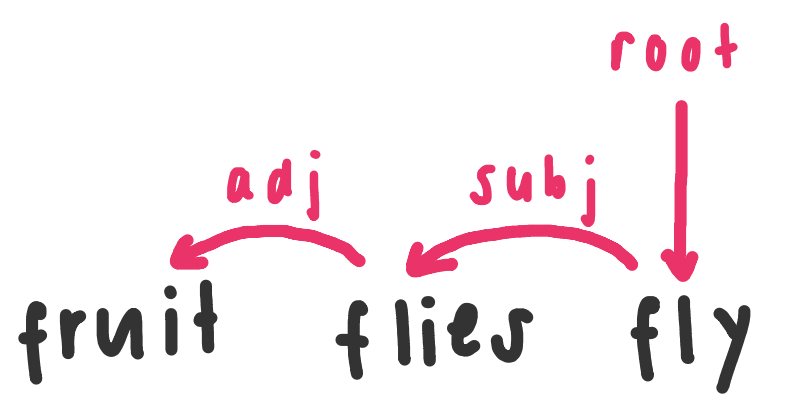
\includegraphics[height=10mm]{inhalt/images/NLP/06_dependency_parsing_1.png}
\\\\
\textit{2) Syntactic parsing $\to$ dependency parsing}\\
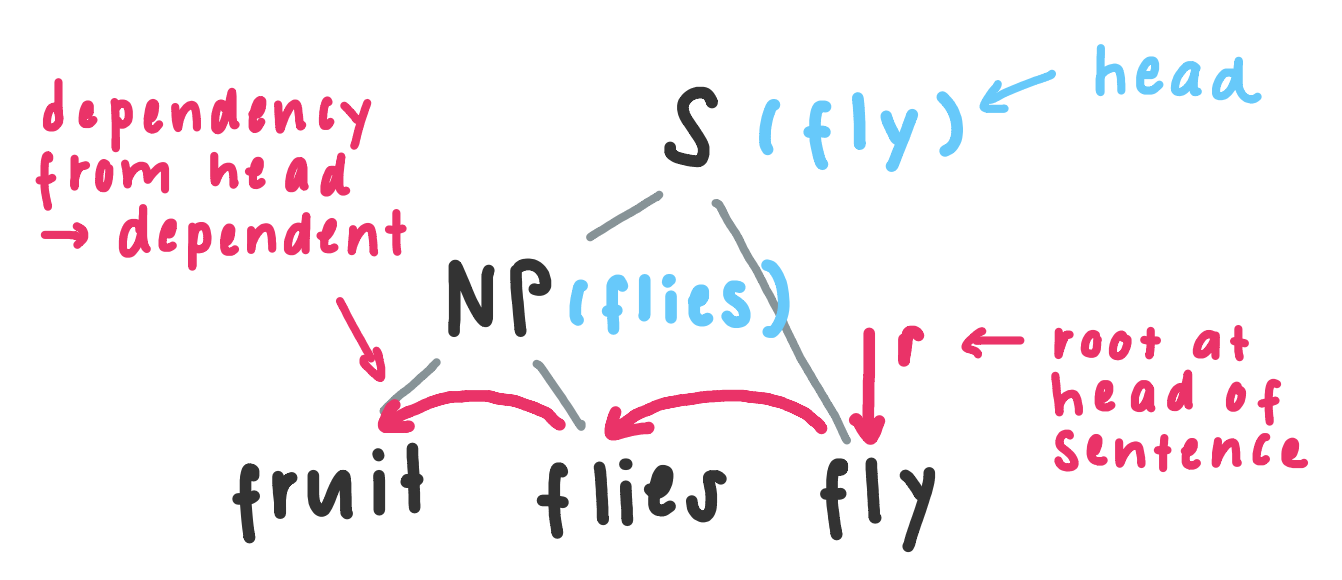
\includegraphics[height=10mm]{inhalt/images/NLP/06_dependency_parsing_2.png}
\end{multicols}